\documentclass[11pt,a4paper]{article}

\usepackage[utf8]{inputenc}
\usepackage[spanish,es-nodecimaldot]{babel}
\usepackage[T1]{fontenc}
\usepackage{lmodern}
\usepackage{geometry}
\geometry{top=2.5cm, bottom=2.5cm, left=2.5cm, right=2.5cm}

\usepackage{amsmath,amssymb}
\usepackage{graphicx}
\usepackage{booktabs}
\usepackage{float}
\usepackage{hyperref}
\hypersetup{colorlinks=true, linkcolor=black, urlcolor=blue}

\setlength{\parindent}{0pt}
\setlength{\parskip}{6pt}

\title{
    \vspace{-1.2cm}
    \textbf{Sistemas de Control}\\
    \large Trabajo de Laboratorio Integrador: Desarrollo de Controladores
}
\author{Tomás Gómez Pizarro \quad\and\quad Mikael Rodríguez}
\date{Noviembre 2026}

\begin{document}

\maketitle

\section*{Primera parte: Control proporcional}

Las especificaciones requeridas para el sistema en lazo cerrado son:
\begin{itemize}
    \item $PO \le 5\%$
    \item $T_s \le 0{,}10\text{ s}$
    \item $e_{ss} = 0$ para escalón unitario
\end{itemize}

\subsection*{Punto 1. Ajuste de $k_p$ mediante el Lugar de las Raíces}

De antemano se observa que la planta es un sistema de \textbf{Tipo 0} (no posee polos en el origen en lazo abierto). Para una entrada escalón unitario, el error en estado estacionario resulta:
\begin{equation}
    e_{ss} = \frac{1}{1 + k_p}
\end{equation}
Para cualquier valor finito de $k_p$, $e_{ss} > 0$. Por lo tanto, la especificación de \textbf{$e_{ss} = 0$ no puede cumplirse} con este controlador.

La función de transferencia de la planta sin considerar la ganancia $k_p$ es:
\begin{equation}
    G(s) = \frac{1}{(0{,}01s + 1)(0{,}0047s + 1)} = \frac{21276{,}6}{(s + 100)(s + 212{,}77)}
\end{equation}

A partir del trazado del Lugar de las Raíces de $G(s)$ y superponiendo la línea de amortiguamiento $\xi = 0{,}69$ (correspondiente al límite de $PO \le 5\%$), se determina mediante la herramienta interactiva el valor de ganancia en la intersección con las ramas:
\begin{equation}
    k_p = 1{,}41
\end{equation}

Para este valor, los polos en lazo cerrado se ubican en $s_{1,2} \approx -156{,}4 \pm j 164{,}0\text{ rad/s}$. Dado que la parte real es $\sigma = -156{,}4\text{ rad/s}$, el tiempo de establecimiento es de aproximadamente $25{,}6\text{ ms}$, cumpliendo holgadamente con $T_s \le 0{,}10\text{ s}$.

\begin{figure}[H]
    \centering
    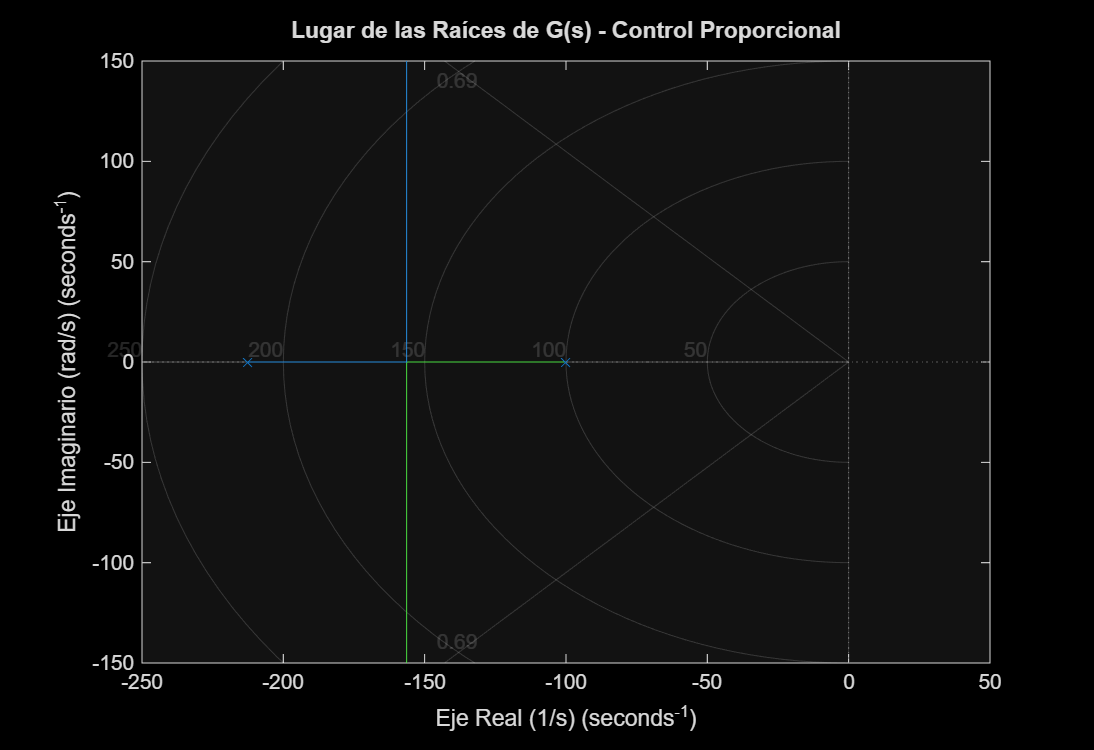
\includegraphics[width=0.7\textwidth]{figuras/punto1_lgr.png}
    \caption{Lugar de las Raíces de $G(s)$, línea de diseño $\xi = 0{,}69$ y polos en lazo cerrado para $k_p = 1{,}41$.}
    \label{fig:punto1_lgr}
\end{figure}

\end{document}
